%Made By Thomas Debelle
\documentclass{report}
\usepackage[a4paper, total={6in, 9in}]{geometry}
\usepackage[utf8]{inputenc}
\usepackage[francais]{babel}
\usepackage{graphicx}
\usepackage{graphics}
\usepackage[T1]{fontenc}
\usepackage{amsmath}
\usepackage{hyperref}
\usepackage{amssymb}
\usepackage{listings}
\usepackage{xcolor}
\usepackage{array}
\usepackage{float}
\usepackage{amsfonts}
\usepackage{fancyhdr}
\usepackage{titlesec}
\usepackage{xparse}
\usepackage{caption}



\newcommand{\undertilde}[1]{\underset{\widetilde{}}{#1}}

\hypersetup{
    colorlinks=true,
    linkcolor=black,
    filecolor=magenta,
    urlcolor=cyan,
    pdftitle={Overleaf Example},
    pdfpagemode=FullScreen,
    }
\begin{document}


\begin{titlepage}
    \begin{figure}
        
\includegraphics[height = 2cm]{Images/UCL_Logo.png}
        \label{fig:my_label}
    \end{figure}

    \hspace*{100cm}
    \centering
    \vspace*{7cm}

    {\Huge \textbf{Résumé de LMECA1901 - MMC}}\\
    \vspace*{0.25cm}
    compilation du \today\\
    \vspace*{0.25cm}
    \Large{Nathan Fockedey, Julien Monfils, Hubert Verheggen\textbf{Ajoutez vos noms si vous participez}}\\

    \vspace*{9cm}
    {\Large Juin 2023}
\end{titlepage}


\tableofcontents
\newpage

\section*{Préface}

Bonjour à toi !\\

Cette synthèse recueille toutes les informations importantes données au cours, pendant les séances de tp et est améliorée grâce au note du Syllabus. Elle ne remplace pas le cours donc écoutez bien les conseils et potentielles astuces que les professeurs peuvent vous donner. Notre synthèse est plus une aide qui, on l'espère, vous sera à toutes et tous utile.\\

Elle a été réalisée par toutes les personnes que tu vois mentionnées. Si jamais cette synthèse a une faute, manque de précision, typo ou n'est pas à jour par rapport à la matière actuelle ou bien que tu veux simplement contribuer en y apportant tes connaissances ? Rien de plus simple ! Améliore la en te rendant \href{http://www.github.com/Tfloow/Q4_EPL}{ici} où tu trouveras toutes les infos pour mettre ce document à jour. (\textit{en plus tu auras ton nom en gros ici et sur la page du github})\\

Nous espérons que cette synthèse te sera utile d'une quelconque manière ! Bonne lecture et bonne étude.

Courage pour l'examen !


\chapter{Introduction}
\section{Objectifs du cours}
La Mécanique des Milieux Continus (MMC) est l'étude de milieux solides ou fluides qui \textbf{se déforment}. Par exemple, la déformation d'une balle lorsqu'on la compresse, le choc entre deux tuyaux, ... La MMC est donc une bonne introduction pour la Mécanique des Fluides et la Mécanique des Solides Déformables car elle va nous donner un tas d'outils mathématiques pour analyser et résoudre des équations de déformations.


\textcolor{red}{à développer}
%TODO

\section{Volumes élémentaires représentatifs}
Lorsqu'on souhaite caractériser une grandeur physique dans un solide complexe (e.g., la masse volumique), on peut utiliser des VER (volumes élémentaires représentatifs). 
\begin{figure}[H]
    \centering
    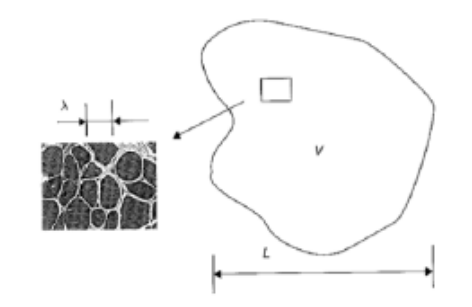
\includegraphics[scale = 0.75]{Images/Images_Introduciton/VER_Schema.png}
    \caption{Illustration d'un VER \protect\footnotemark}
    \label{fig:my_label}
\end{figure}
\footnotetext{Image tirée des slides "introduction", version 2017}
Le principe est le suivant : On prend un "petit morceau" du volume afin de représenter les propriétés moyennes du matériau. Ce morceau doit être suffisamment grand pour qu'il  représente correctement la structure du matériau et assez petit que pour qu'il puisse être mathématiquement considéré comme un point mais pas comme une molécule ou un atome.

\begin{figure}[H]
    \centering
    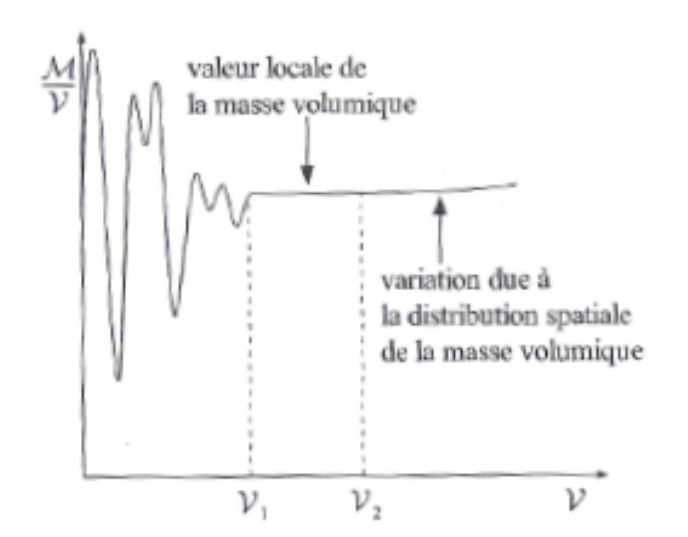
\includegraphics[scale = 0.5]{Images/Images_Introduciton/VER_Graphe.png}
    \caption{Fluctuation de la masse volumique en fonction du volume de l'élément \protect \footnotemark}
    \label{fig:fluctuationsVER}
\end{figure}
\footnotetext{Image tirée des slides "introduction", version 2017}

Pour trouver la grandeur en un point du solide, on fera la moyenne de cette grandeur sur un élément de volume l'entourant. De plus, dans cette moyenne, on se servira du modèles à une échelle inférieur. (e.g., échelle cristalline, moléculaire)\\
\\
Par exemple : Si nous souhaitons calculer la masse volumique d'un solide en un point P.
\begin{enumerate}
    \item On choisi un élément de volume de taille adéquate
    \item On calcul la moyenne de la masse volumique sur cet élément de volume en suivant le modèle cristallin
    \item La masse volumique du solide au point P vaudra la moyenne calculée à l'étape 2.
\end{enumerate}
Comme on le voit sur la figure \ref{fig:fluctuationsVER}, Si le volume de l'élément est inférieur à $V_1$, la masse volumique de l'élément ne sera plus représentative de la masse volumique du solide. Pour une faible variation de volume, la masse volumique variera de manière non-négligeable. En revanche, si le volume est supérieur à $V_1$, la masse volumique sera presque constante. Il nous faut donc choisir une taille de VER telle que $\lambda << VER << V$, où $\lambda$  est de taille infiniment petite et V est le volume total de notre Milieu Continu.\\

\section{Les hypothèses de la MMC}

\begin{itemize}
    \item Les lois ne sont pas modifiées si on change d'observateur
    \item Les lois ne sont pas modifiées si on change le systèmes de coordonnées.
    \item Les lois sont les mêmes partout dans l'espace et dans le temps.
    \item L'espace est euclidien ($\mathbb{R}^3$ muni d'un produit scalaire)
\end{itemize}




\chapter{Notions d'algèbre}
\section{Vecteurs}
\subsection{Base orthonormée}
On dit qu'une base $(e_1, e_2, e_3)$ est orthonormée si
\begin{equation*}
    \textbf{e}_i \cdot \textbf{e}_j = \delta_{ij}
\end{equation*}
Où $\delta_{ij}$ est le symbole de Kronencker. Il est défini comme suit

\begin{equation*}
    \delta_{ij} = 
    \begin{cases}
        1 & \text{ si $i = j$}\\
        0 & \text{ si $i \neq j$}\\
    \end{cases}
\end{equation*}\\
Dans ce cours, uniquement les bases orthonormées seront considérées.

\subsection{Notation d'Einstein}

Afin de simplifier les notations, nous utiliserons dans ce cours la notation de Einstein. Celle-ci permet de simplifier l'écriture des sommes.\\

Lorsqu'on est face à une expression faisant intervenir des indices, il faut distinguer les indices \textbf{répétés} et les indices \textbf{muets}.\\
\\
Prenons l'expression suivantes :
\begin{equation*}
    u_j = \alpha v_j
\end{equation*}
Ici, l'indice $j$ est considéré comme muet. Il intervient \textbf{des deux côtés de l'égalité}\\
\\
En revanche, si on écrit l'égalité suivante :
\begin{align*}
    \Vec{\mathbf{u}} &= \sum_i u_i \mathbf{\hat{e}_i}\\
    \vec{\mathbf{u}} &= u_i \mathbf{\hat{e}_i}
\end{align*}
L'indice $i$ est dit répété. En effet, il n'apparaît que d'un côté de l'égalité. Cette notation $\vec{\mathbf{u}} &= u_i \mathbf{$\hat{e}_i$}$ sous-entend en fait la somme pour $i = 1, 2, 3$


\subsection{Changement de base}

Soit une base $(\textbf{e}_i)$ et une base $(\textbf{e}_i')$ et soit $\textbf{P} \in \mathbb{R}^{3\times 3}$ la matrice de changement de base.\\

On a 
\begin{equation*}
    \textbf{e}_i' = P_{ij}e_j
\end{equation*}



\section{Tenseurs}

Un tenseur est un objet mathématique, étendant les concepts de scalaire et de vecteur, qui peut être représenté par ses composantes dans une base donnée. Cet objet se doit également d'obéir à des règles précises de transformation lors d'un changement de base.
\subsection{Pourquoi utiliser des tenseurs ?}
Pour caractériser les certaines propriétés telles que la déformation ou les contraintes, nous avons besoin de connaître 6 informations pour un point de l'espace (trop pour un vecteur). Il est donc nécessaire de généraliser le concept de vecteur et arriver aux tenseurs.

\subsection{Représentation (notation) des tenseurs}
Tout d'abord, il faut toujours garder en tête qu'\textbf{un tenseur est exprimé dans une base}\\

Un tenseur peut s'exprimer de plusieurs façons différentes : 
\begin{itemize}
    \item De manière indicielle : $\mathbf{\undertilde{a}} = (a_{ij}) \text{ in } (\mathbf{\hat{e}_i})$
    \item De manière matricielle :  $\mathbf{\undertilde{a}} = [a] \text{ in } (\mathbf{\hat{e}_i})$
\end{itemize}


\subsection{Opérations sur les tenseurs}
\begin{itemize}
    \item Le produit tensorielle de deux vecteurs : 
    \begin{equation*}
        \mathbf{\undertilde{a}} = \vec{\mathbf{u}} \otimes \vec{\mathbf{v}} \text{ où, } a_{ij} = u_i v_j \text{ in } (\mathbf{\hat{e}_i})
    \end{equation*}
    Le produit tensoriel peut s'exprimer de manière matricielle comme suit 
    \begin{equation*}
        \mathbf{\undertilde{a}} = \{\mathbf{u}\} \{\mathbf{v}\} ^T
    \end{equation*}
    Où $\mathbf{u}$ et $\mathbf{v}$ sont deux vecteurs colonnes.\\

    \textbf{Conséquence} : N'importe quel tenseur $\mathbf{\undertilde{a}}$ peut se décomposer comme suit : 
    \begin{equation*}
    \mathbf{\undertilde{T}} = a_{ij} \mathbf{\hat{e}_i} \otimes \mathbf{\hat{e}_j}
\end{equation*}

\item Le produit entre tenseur et vecteur : 
    \begin{equation*}
        \Vec{\mathbf{v}} = \mathbf{\undertilde{a}}(\Vec{\mathbf{u}}) = \mathbf{\undertilde{a}} \cdot \Vec{\mathbf{u}} \text{ où, } v_i = a_{ij} v_j
    \end{equation*}

\item La trace d'un tenseur : 
    \begin{equation*}
        tr(\mathbf{\undertilde{a}}) = a_{ii}
    \end{equation*}

\item Le produit contracté sur un indice :\\

    Entre un tenseur $\mathbf{\undertilde{a}}$ et un vecteur $\Vec{\mathbf{v}}$ :
    \begin{equation*}
        (\mathbf{\undertilde{a}} \cdot \Vec{\mathbf{v}})_i = a_{ij}v_j
    \end{equation*}

    Entre un tenseur $\mathbf{\undertilde{a}}$ et un tenseur $\mathbf{\undertilde{b}}$ : 

    \begin{equation*}
        (\mathbf{\undertilde{a}} \cdot \mathbf{\undertilde{b}})_{ij} = a_{ik}b_{kj}
    \end{equation*}

\item Le produit contracté sur deux induces : 
    \begin{equation*}
        \mathbf{\undertilde{a}} : \mathbf{\undertilde{b}} = a_{ij}b_{ji} = tr(\mathbf{\undertilde{a}} \cdot \mathbf{\undertilde{b}})
    \end{equation*}
\end{itemize}


\subsection{Les tenseurs symétriques}

Un tenseur symétrique $\mathbf{\undertilde{a}}$ peut être décomposé en une composante déviatorique et une composante sphérique.


\begin{equation*}
    \mathbf{\undertilde{a}} = \underbrace{\mathbf{\undertilde{a}} - \frac{1}{3} tr(\mathbf{\undertilde{a}}) \mathbf{\undertilde{1}}}_{deviatoriµque} + \underbrace{\frac{1}{3} tr(\mathbf{\undertilde{a}})\mathbf{\undertilde{1}}}_{spherique}
\end{equation*}

Cette décomposition sera utile plus tard pour représenter respectivement des changement de forme et des changements de volume.

\subsection{Les invariants}

Les invariants sont des propriétés d'un tenseur qui \textbf{ne dépendent pas} de la base dans laquelle il est exprimé.\\

\textit{Pour vérifier si on n'a pas fait d'erreur dans un changement de base, il suffit de vérifier que les invariants sont conservés.}\\

Les invariants d'un tenseur sont : 
\begin{itemize}
    \item La trace 
    \item Le déterminant
\end{itemize}

\chapter{Cinématique}
\section{Référence et états}
Considérons un solide qui subit une déformation. Celui-ci possède un état initial $\Omega_0$ et un état final $\Omega_t$ 

\begin{figure}[H]
    \centering
    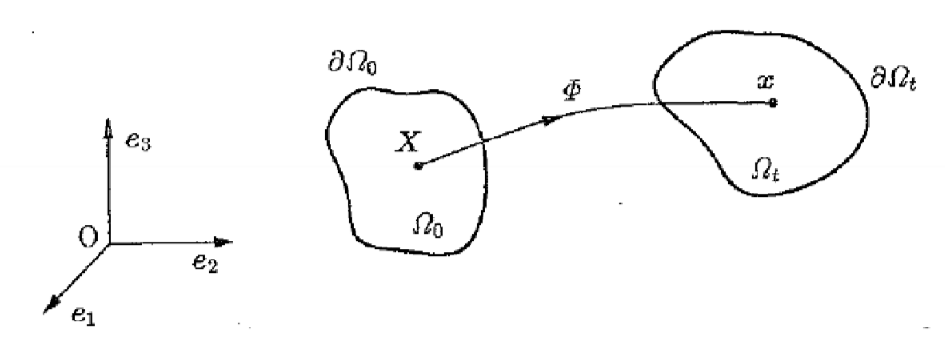
\includegraphics[width = 8cm]{Images/Cinematique/Etats1.png}
    \label{fig:my_label}
\end{figure}
Considérons une particule de ce solide. Son vecteur position est $\mathbf{X}$ dans $\Omega_0$ et $\mathbf{x}$ dans $\Omega_t$.\\
On défini la transformation $\mathbf{\Phi} : \Omega_0 \rightarrow \Omega_t \; \mathbf{X} \rightarrow \mathbf{x} = \mathbf{\Phi}(\textbf{X},t)$

\subsection{Description eulérienne et lagrangienne}

Il existe deux manières de décrire un phénomène en MMC : \\
\begin{itemize}
    \item La description lagrangienne (matérielle) : On place l'observateur sur une particule de matière et on s'intéresse à \textit{comment celle-ci perçoit le champ vectoriel étudié.}\\

    \textit{Exemple : On pose une brindille dans une rivière et on voit comment se déplace la brindille.}\\
    
    \item La description eulérienne (spatiale) : On place l'observateur à un endroit fixe et il observe les particules qui passent sous ses yeux.\\
    
    \textit{Exemple : On donne le champ de vitesse dans un fluide qui s'écoule. En tout point on connaît la vitesse d'une particule.}
\end{itemize}

\subsubsection{Lien entre la description lagrangienne et eulérienne}

\textcolor{red}{Je ne sais pas trop si il faut faire le lien entre les deux description, ou juste évoquer la dérivée langrangienne et l'expliquer (ce que je voulais faire de base)}

Si on étudie une grandeur avec une description lagrangienne, il faut faire attention en la dérivant. Considérons la grandeur $\mathbf{K}(\mathbf{X}, t)$, calculons sa dérivée temporelle.
\begin{equation*}
    \frac{\partial}{\partial t} \mathbf{K}(\mathbf{X}, t) = \frac{\partial \mathbf{k}}{\partial t} + \frac{\partial \mathbf{k}}{\partial \mathbf{x}} \frac{\partial  \mathbf{x}}{\partial t} = \frac{\partial \mathbf{k}}{\partial t} + \underbrace{\frac{\partial \mathbf{k}}{\partial \mathbf{x}}}_{\nabla \mathbf{k}} \mathbf{v}(\mathbf{x}, t) \equiv \frac{\mathcal{D} k}{\mathcal{D} t}
\end{equation*}

\textcolor{red}{Je suis peut être le seul à avoir galéré à comprendre ça (l'interprétation physique), du coup dites moi si c'est pertinent ou non, auquel cas on peut l'enlever. (Julien Monfils)}\\

\textit{Interprétation physique :}
\\

\textit{
Plaçons un observateur sur une particule traversant un champ de température qui ne varie pas dans le temps} $(\frac{\partial k}{\partial t} = \frac{\partial T}{\partial t} = 0)$.\\

%Y a une erreur Latex ici, jsp pourquoi
\textit{On s'intéresse maintenant à la dérivée de la température mesurée par l'observateur. Selon la formule développée ci-dessus, on a}
\begin{equation*}
    \frac{\mathcal{D} T}{\mathcal{D} t} = \nabla T \cdot \mathbf{v}(\mathbf{x}, t)
\end{equation*}
\textit{La relation de proportionnalité entre la dérivée temporelle de $T$ et la vitesse de la particule peut s'expliquer de la manière suivante :}\\

\textit{Si l'observateur ne se déplace pas dans le champs de température, il ne perçoit aucune variation de température, la dérivée temporelle est donc nulle.}\\

\textit{Si l'observateur est mobile, la dérivée temporelle sera proportionnelle à la vitesse. En effet, plus il se déplacera vite, plus les changements de températures qu'il percevra seront rapides.}

\section{Gradient de déformation}
\end{document}
